\documentclass[../sherrill-Mix_thesis.tex]{subfiles}
\begin{document}
\chapter{Conclusions and future directions}
\graphicspath{{im/}{conclusion/im/}}

In this dissertation, we described studies to characterize the nature of HIV-1 latency, expression and alternative splicing and host cells' response to infection.

\section{Latency and integration location}

The chromosomal location of integration was shown to affect proviral latency but the mechanisms appear to differ between cell culture models. This suggests that 

%http://journals.plos.org/plospathogens/article?id=10.1371/journal.ppat.1003834

Further clarification using more detailed sequencing in more time points, cell types and strains of HIV-1 and other lentiviruses rema

A common theme was that cell lines and \textit{in vitro} models of these replication steps often disagree with each other and with primary cell data. 

PacBio was bad. Figure? Do better

Comparison among labs and cell types/viruses at same time. Standardize.

Non polyadenylated RNA. Strand specific sequencing. Longer reads and longer fragments.

\section{HIV-1 alternative splicing}
In addition an important subset of HIV are the founder viruses transmitted between hosts \citep{Keele2008,Salazar-Gonzalez2009}. These viruses are not well studied and perhaps their splicing and gene expression differ from the rest of the viral swarm of late-term patients.

\section{Host expression during HIV infection}

Cell lines bad

Endogenous retrovirus

\section{LAMP PCR and lab-on-a-chip}
	In Chapter \ref{chapLamp}, we report primers optimized to detect most subtypes of HIV-1. An interesting alternative to picking up all subtypes with a single primer would be to design primers targeted specifically to each subtype so that a positive amplification would then be able to discriminate viral subtype.

	In a recent outbreak in West Africa, Zaire ebolavirus has infected over 26,000 confirmed, probable and suspected cases and caused over 11,000 reported deaths \citep{Gire2014,WHOERT2014,WHO2015}. Early detection and quarantine are essential to the control of this epidemic \citep{Chowell2014}. Amplification of Ebola virus nucleic acid through polymerase chain reaction is the best diagnostic test currently available but the necessary resources are often not available in these resource-poor regions \citep{Fauci2014,WHO2015a}. Antigen-based tests are quicker and available at the point-of-care but are not as accurate or sensitive as polymerase chain reaction tests and are still in limited supply \citep{WHO2015a}.

	Loop-mediated isothermal amplification (LAMP) offers the potential to allow rapid, sensitive and efficient detection of Ebola RNA but currently available LAMP primers \citep{Kurosaki2007} do not match this viral strain. Using sequences from the recent outbreak \citep{Gire2014,Hoenen2015} and the methods described in Chapter \ref{chapLamp}, we designed primers to match all known Zaire ebolavirus \ref{figEbolaConsensus}. These primer combined with simple lab-on-a-chip devices for purifying blood plasma \citep{Liu2013} and imaging fluorescent signals \citep{Liu2011} could allow rapid point-of-care detection of Ebolavirus.

	\begin{figure}
		\centering
		%%[[FIX THIS FIGURE and name Ebola right]]
		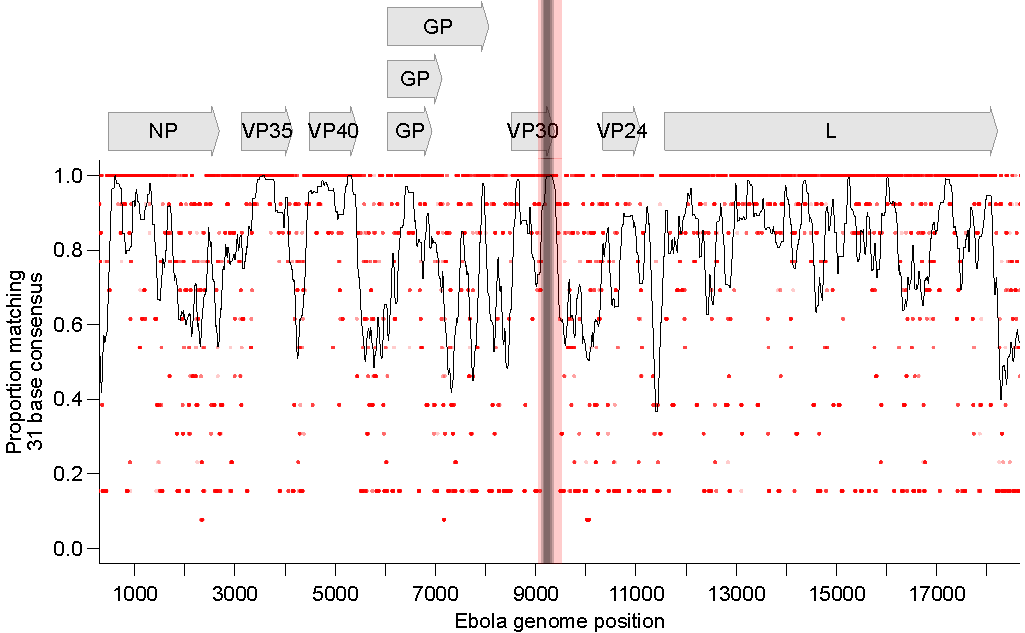
\includegraphics[width=.6\textwidth]{ebolaConsensus.pdf} %REMOVE%
		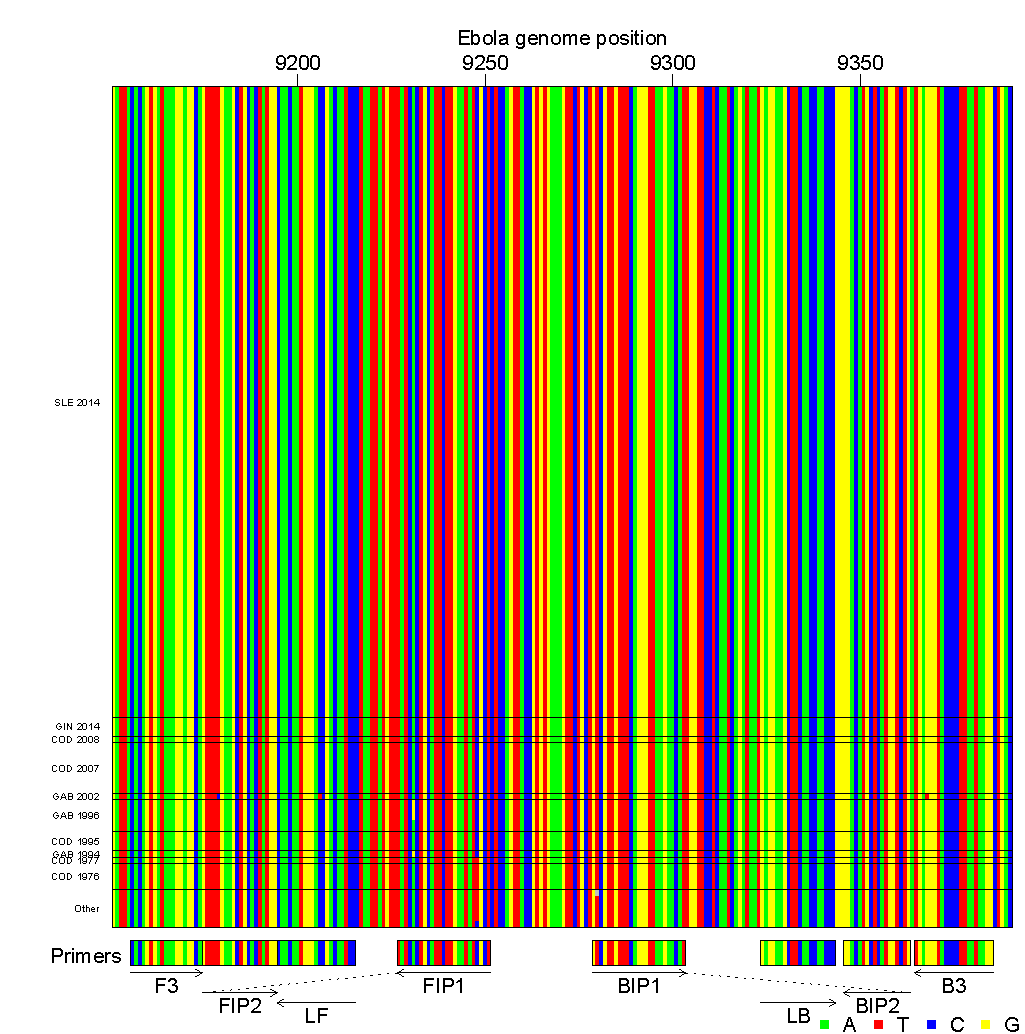
\includegraphics[width=.6\textwidth]{loop_bases.pdf} %REMOVE%
		\caption[Ebola RT-LAMP primers design]{Bioinformatic analysis to design Ebola RT-LAMP primers. A) Conservation of sequence in Ebola. Ebola genomes (n = 131) from Genbank and sequences from the recent Zaire Ebolavirus outbreak \citep{Gire2014} were aligned and conservation calculated. The x-axis shows the coordinate on the Ebola genome, the y-axis shows the proportion of sequences matching the consensus for each 21 base segment of the genome (red points). The black line shows a 101 base sliding average over these proportions. The vertical red shading shows the region targeted for LAMP primer design that was used as input into the EIKEN primer design tool. Numbering is relative to the Ebola Mayinga sequence. B) Aligned genomes, showing the locations of the preliminary primers. Sequences in the red shaded region in A are shown, with DNA bases color-coded as shown at the lower right. Each row indicates an HIV sequence and each column a base in that sequence. Horizontal lines separate Ebolavirus outbreaks (labeled at left). Arrows indicate the strand targeted by each primer. Primers targeting the negative strand of the virus are shown as reverse compliments for ease of viewing.}
		\label{figEbolaConsensus}
	\end{figure}


\end{document}
